VISOR software is not officially supported by the KR1410 and there is no direct integration of the VISOR camera available.
However, Kassow robots provides support to build own software through CBun development.
The CBun (Capability Bundle) represents a modular framework within the KR software system,
which encapsulates functionalities and provides the
access to its predefined \hyperref[acro:API]{API}. 


\begin{figure}[h]
    \centering
    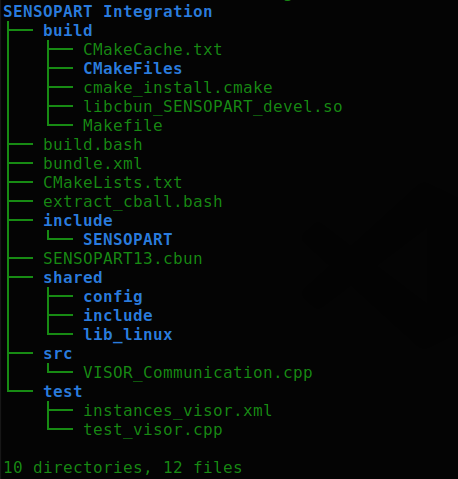
\includegraphics[width=0.44\textwidth]{figures/sensopart-development.png}
    \caption{CBun Project Setup for SENSOPART Integration in KR}
    \label{fig:sensopart-development}
\end{figure}


The CBun SDK is the Software Development Kit that provides all essential tools
for CBun development. The project setup is created in a Visual Studio Code container
running on Ubuntu 18.04 with a special set of software packages. \cite{Cbun}
The header files are located in \textbf{include} directory and C++ source file \textit{i.e.}     \textit{VISOR\_Communication.cpp}
are placed in \textbf{src} directory.
Upon building the project, a SENSOPART.cbun file is generated as shown in \ref{fig:sensopart-development}
It is then installed in the teach pendant using a \hyperref[acro:USB]{USB}. Figure \ref{fig:cbun-variables}
shows the information of VISOR variables getting through the VISOR to KR1410.

\begin{figure}[h]
    \centering
    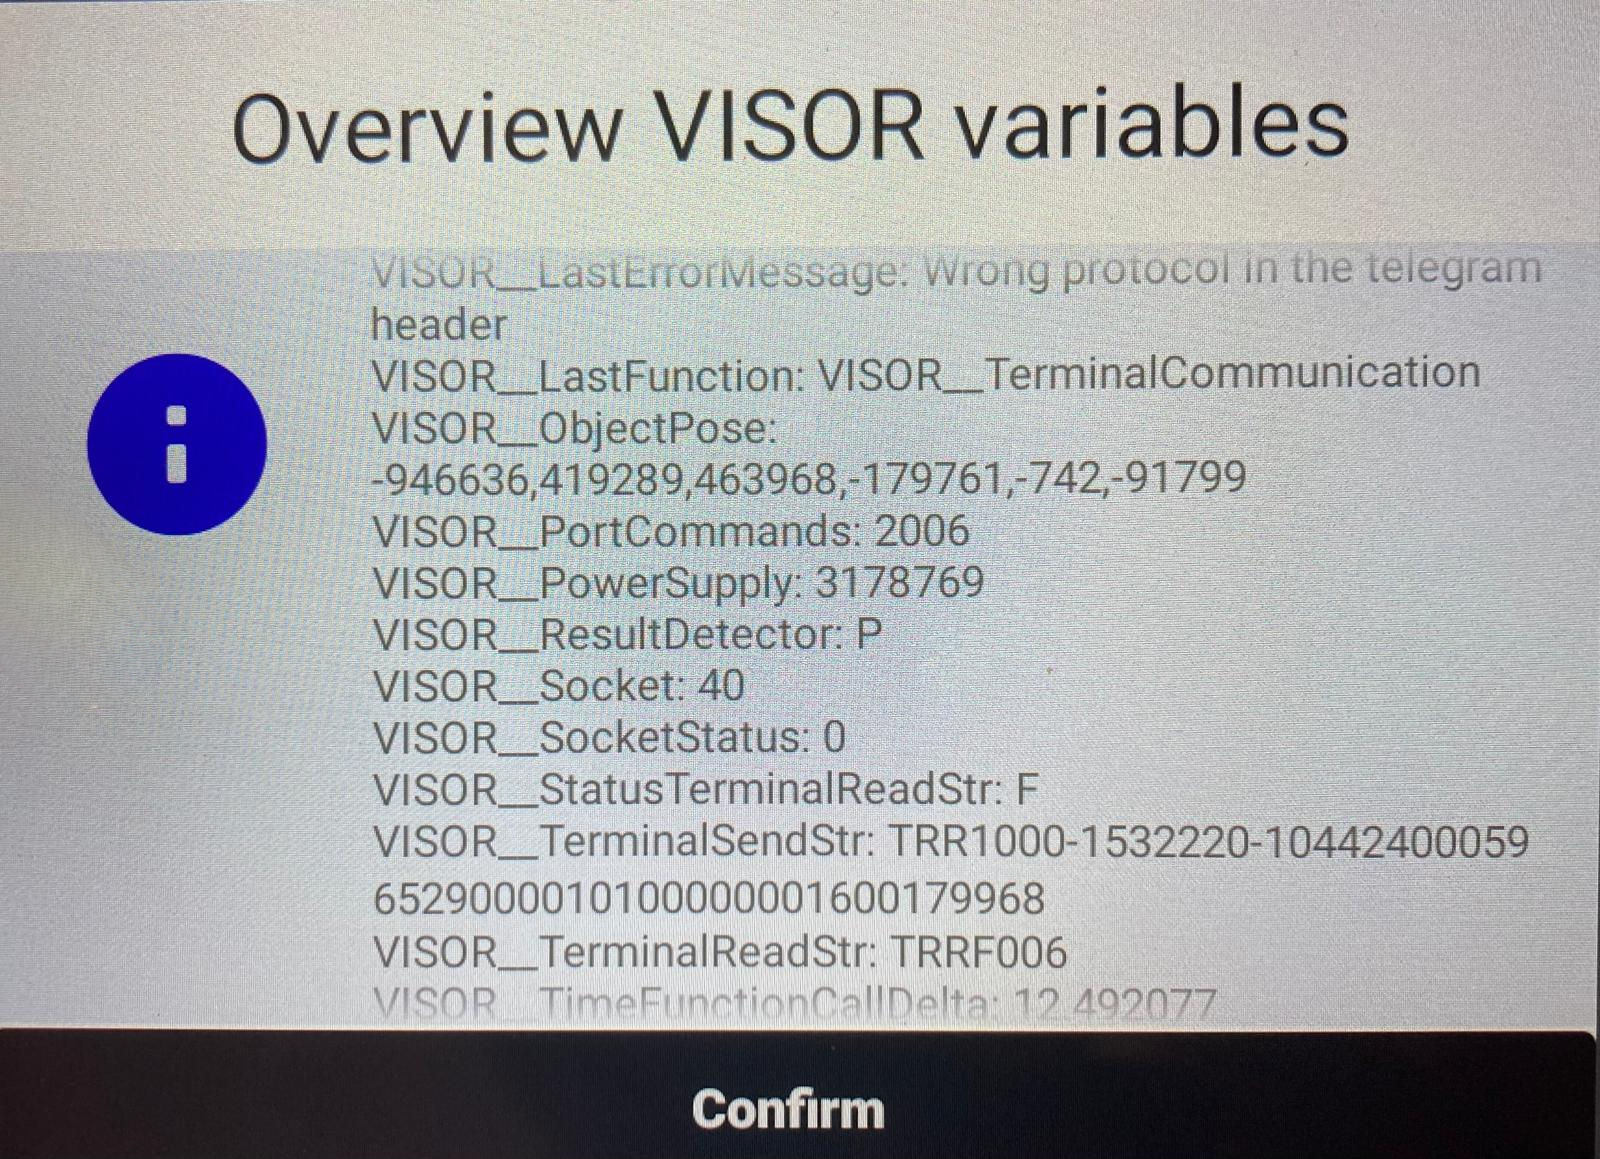
\includegraphics[width=0.55\textwidth]{figures/visor-cbun-connection.png}
    \caption{Dialog Box showing current VISOR variables}
    \label{fig:cbun-variables}
\end{figure}

CBun device is one of the CBun elements. CBun Device concept allows to wrap handling code of physical device like VISOR vision sensor into the CBun and hide it from the end user. This allows the user to simply control and monitor devices without the need to implement the communication and logic. \cite{cbun-device}

VISOR camera is powered from the TPSU02 on the KR1410 tool-IO.
A CBun device named VISOR from CBun developement is created which has methods for
controlling the functionalities of camera like changing job, getting object pose by triggering camera and performing calibration. Through this
device, the KR communicates with the VISOR over telegram.

